% ============================================================
%  Curriculum Vitae - Ronald J. Tackett, Ph.D.
%  Engine: XeLaTeX
%
%  CHANGELOG
%  v1.1  2026-09-04  Corrected two publication entries: Bi2Ti2O7 (was O4)
%                    and 'La- and Dy-doped ... ferrimagnetic' (was Hy /
%                    ferromagnetic), verified against the AIP record.
%  v1.0  2026-09-03  Rebuilt in LaTeX from the March 2026 PDF.
%                    Changes relative to that version:
%                      - Added two invited talks (CoLLT, Georgia Tech,
%                        April 10 2026 and September 4 2026)
%                      - Added Treasurer and Past Chair, EGLS APS
%                      - Added Founding Member, CoLLT
%                      - Added Google Scholar and ORCID to contact block
%                      - Footer date to September 3, 2026
% ============================================================
\documentclass[10pt]{article}
\usepackage{tackettdoc}

\setdoclabel{Ronald J. Tackett, Ph.D. \textperiodcentered\ Curriculum Vitae}
\setupdated{September 3, 2026}

\begin{document}

% ── HEADER ──────────────────────────────────────────────────
\begin{minipage}[t]{\dimexpr\textwidth-1.55in\relax}
  \vspace{0pt}
  {\color{accent}\fontsize{25}{28}\selectfont\robotolight Ronald J.\ \textbf{\rmfamily\bfseries Tackett, Ph.D.}\par}
  \vspace{0.3em}
  {\color{subtext}\fontsize{10}{13}\selectfont\bfseries Founding Head of School \& Associate Professor of Physics\par}
  {\color{mutedtext}\fontsize{9.5}{12}\selectfont\robotolight School of Foundational Studies \textperiodcentered\ Kettering University\par}
\end{minipage}%
\hfill
\begin{minipage}[t]{1.45in}
  \vspace{0pt}
  \raggedleft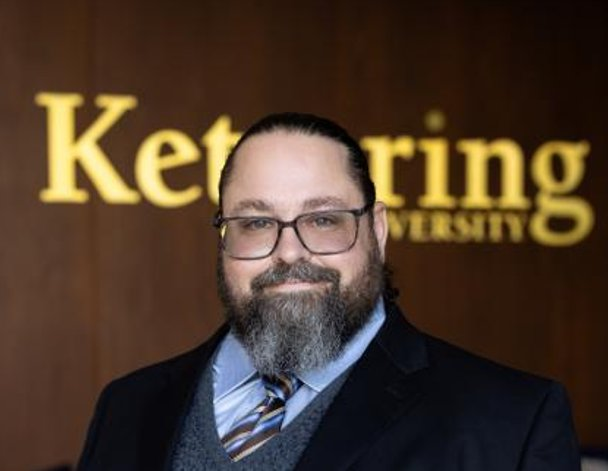
\includegraphics[width=1.15in]{headshot.jpg}
\end{minipage}

\vspace{1.0em}
{\color{rulelight}\hrule height 0.5pt}
\vspace{0.9em}

\begin{center}
  {\fontsize{9.5}{13}\selectfont
   \href{mailto:rtackett@kettering.edu}{rtackett@kettering.edu} \quad|\quad
   \href{https://linkedin.com/in/rtackett30}{linkedin.com/in/rtackett30} \quad|\quad
   \href{https://rtackett30.github.io}{rtackett30.github.io}\par
   1700 University Ave, Flint, MI 48504 \quad|\quad
   \href{https://rtackett1978.wordpress.com}{rtackett1978.wordpress.com}\par
   ORCID: \href{https://orcid.org/0000-0001-9611-4368}{0000-0001-9611-4368} \quad|\quad
   \href{https://scholar.google.com/citations?user=7EFWzPsAAAAJ&hl=en}{Google Scholar}\par}
\end{center}

\vspace{0.9em}
{\color{accent}\hrule height 1.6pt}

% ── EDUCATION ───────────────────────────────────────────────
\cvsection{Education}

\cventry{Ph.D., Condensed Matter Physics}{Wayne State University, Detroit, MI}{2003--2008}
\vspace{-0.15em}
\begin{itemize}[leftmargin=1.2em, itemsep=0.05em, topsep=0.1em, parsep=0pt]
  \fontsize{9}{11}\selectfont
  \item Dissertation: \textit{The Synthesis, Characterization, and Application of Multifunctional Magnetic Nanoparticles}
  \item Advisor: Dr.\ Gavin Lawes
\end{itemize}
\vspace{0.5em}

\cventry{B.S., Engineering Physics}{Eastern Michigan University, Ypsilanti, MI}{2001--2003}

% ── PROFESSIONAL EXPERIENCE ─────────────────────────────────
\cvsection{Professional Experience}

\cventry{Founding Head (Dean-Equivalent), School of Foundational Studies}{Kettering University, Flint, MI}{2025--pres.}
\cventry{Adjunct (Volunteer) Associate Professor of Physics}{Wayne State University, Detroit, MI}{2025--pres.}
\cventry{Associate Professor of Physics}{Kettering University, Flint, MI}{2019--pres.}
\cventry{Assistant Professor of Physics}{Kettering University, Flint, MI}{2014--2019}
\cventry{Assistant Professor of Physics}{Arkansas Tech University, Russellville, AR}{2010--2014}
\cventry{Postdoctoral Research Associate}{University of Texas at El Paso, El Paso, TX}{2008--2010}
\cventry{Graduate Research Assistant}{Wayne State University, Detroit, MI}{2004--2008}
\cventry{Graduate Teaching Assistant}{Wayne State University, Detroit, MI}{2003--2004}

% ── PUBLICATIONS ────────────────────────────────────────────
\cvsection{Publications}

\cvsubsection{Published}

\begin{reflist}
\item B.R. Dahal, K. Schroeder, M.M. Allyn, \textbf{R.J. Tackett}, Y. Huh, and P. Kharel. ``Near-room-temperature magnetocaloric properties of La$_{1-x}$Sr$_x$MnO$_3$ ($x$ = 0.11, 0.17, and 0.19) nanoparticles.'' \textit{Mat.\ Res.\ Express} \textbf{5}, 106103 (2018). \href{https://doi.org/10.1088/2053-1591/aadabd}{\small\allowbreak doi:10.1088/2053-1591/aadabd}
\item \textbf{R.J. Tackett}, J. Thakur, N. Mosher, E. Perkins-Harbin, R.E. Kumon, L. Wang, C. Rablau, and P.P. Vaishnava. ``A method for measuring the N\'eel relaxation time in a frozen ferrofluid.'' \textit{J.\ Appl.\ Phys.} \textbf{118(6)}, 064701 (2015). \href{https://doi.org/10.1063/1.4928202}{\small\allowbreak doi:10.1063/1.4928202}
\item Y.C.N. Chen, C.Y. Hsieh, \textbf{R. Tackett}, P. Kokeny, R.K. Regmi, and G. Lawes. ``Magnetic moment quantifications of small spherical objects in MRI.'' \textit{Mag.\ Res.\ Imaging} \textbf{33(6)}, 829 (2015). \href{https://doi.org/10.1016/j.mri.2014.11.003}{\small\allowbreak doi:10.1016/j.mri.2014.11.003}
\item C.E. Botez, A.H. Adair, and \textbf{R.J. Tackett}. ``Evidence of superspin-glass behavior in Zn$_{0.5}$Ni$_{0.5}$Fe$_2$O$_4$ nanoparticles.'' \textit{J.\ Phys.\ Cond.\ Mat.} \textbf{27(7)}, 076005 (2015). \href{https://doi.org/10.1088/0953-8984/27/7/076005}{\small\allowbreak doi:10.1088/0953-8984/27/7/076005}
\item S.S. Laha, \textbf{R.J. Tackett}, and G. Lawes. ``Interactions in $\gamma$-Fe$_2$O$_3$ and Fe$_3$O$_4$ nanoparticle systems.'' \textit{Physica B} \textbf{448}, 69 (2014).
\item C.E. Botez, \textbf{R.J. Tackett}, J.D. Hermosillo, J.Z. Zhang, Y.S. Zho, and L.P. Wang. ``High-pressure synchrotron x-ray diffraction studies of superprotonic transitions in phosphate solid acids.'' \textit{Solid State Ionics} \textbf{213}, 58 (2012). \href{https://doi.org/10.1016/j.ssi.2011.08.015}{\small\allowbreak doi:10.1016/j.ssi.2011.08.015}
\item \textbf{R. Tackett}, G. Lawes, R. Suryanarayanan, M. Apostu, and A. Revcolevschi. ``The zero-field glassy ground state and field-induced ferromagnetic transition in (La$_{0.4}$Pr$_{0.6}$)$_{1.2}$Sr$_{1.8}$Mn$_2$O$_7$.'' \textit{J.\ Phys.\ Cond.\ Mat.} \textbf{23}, 156004 (2011). \href{https://doi.org/10.1088/0953-8984/23/15/156004}{\small\allowbreak doi:10.1088/0953-8984/23/15/156004}
\item K.K. Bharathi, \textbf{R.J. Tackett}, C.E. Botez, and C.V. Ramana. ``Coexistence of spin glass behavior and long-range ferrimagnetic ordering in La- and Dy-doped Co ferrite.'' \textit{J.\ Appl.\ Phys.} \textbf{109}, 07A510 (2011). \href{https://doi.org/10.1063/1.3562201}{\small\allowbreak doi:10.1063/1.3562201}
\item C.E. Botez, A.W. Bhuiya, and \textbf{R.J. Tackett}. ``Dynamic-susceptibility studies of the interplay between the N\'eel and Brown magnetic relaxation mechanisms.'' \textit{App.\ Phys.\ A} \textbf{104}, 177 (2011). \href{https://doi.org/10.1007/s00339-010-6098-x}{\small\allowbreak doi:10.1007/s00339-010-6098-x}
\item C.E. Botez, D. Carbajal, K. Adiraju, and \textbf{R.J. Tackett}. ``Intermediate-temperature polymorphic phase transition in KH$_2$PO$_4$: A synchrotron x-ray diffraction study.'' \textit{J.\ Phys.\ Chem.\ Sol.} \textbf{71}, 1576 (2010). \href{https://doi.org/10.1016/j.jpcs.2010.08.004}{\small\allowbreak doi:10.1016/j.jpcs.2010.08.004}
\item \textbf{R.J. Tackett}, J.G. Parsons, B.I. Machado, S. Gaytan, L.E. Murr, and C.E. Botez. ``Evidence of low-temperature superparamagnetism in Mn$_3$O$_4$ nanoparticle ensembles.'' \textit{Nanotechnology} \textbf{21}, 365703 (2010). \href{https://doi.org/10.1088/0957-4484/21/36/365703}{\small\allowbreak doi:10.1088/0957-4484/21/36/365703}
\item \textbf{R.J. Tackett}, A.W. Bhuiya, and C.E. Botez. ``Dynamic susceptibility evidence of surface spin freezing in ultrafine NiFe$_2$O$_4$ nanoparticles.'' \textit{Nanotechnology} \textbf{20}, 445705 (2009). \href{https://doi.org/10.1088/0957-4484/20/44/445705}{\small\allowbreak doi:10.1088/0957-4484/20/44/445705}
\item C.E. Botez, H. Martinez, \textbf{R.J. Tackett}, R.R. Chianelli, J. Zhang, and Y. Zhao. ``High-temperature crystal structures and chemical modifications in RbH$_2$PO$_4$.'' \textit{J.\ Phys.\ Cond.\ Mat.} \textbf{21}, 325401 (2009). \href{https://doi.org/10.1088/0953-8984/21/32/325401}{\small\allowbreak doi:10.1088/0953-8984/21/32/325401}
\item K. Senevirathne, \textbf{R. Tackett}, P.R. Kharel, G. Lawes, K. Somaskandan, and S.L. Brock. ``Discrete, dispersible MnAs nanocrystals from solution methods: phase control on the nanoscale and magnetic consequences.'' \textit{ACS Nano} \textbf{3}, 1129 (2009). \href{https://doi.org/10.1021/nn900194f}{\small\allowbreak doi:10.1021/nn900194f}
\item R. Regmi, \textbf{R. Tackett}, and G. Lawes. ``Suppression of low-temperature magnetic states in Mn$_3$O$_4$ nanoparticles.'' \textit{J.\ Magn.\ Magn.\ Mater.} \textbf{321}, 2296 (2009). \href{https://doi.org/10.1016/j.jmmm.2009.01.041}{\small\allowbreak doi:10.1016/j.jmmm.2009.01.041}
\item B.C. Melot, \textbf{R. Tackett}, J. O'Brien, A.L. Hector, G. Lawes, R. Seshadri, and A.P. Ramirez. ``Large low-temperature specific heat in pyrochlore Bi$_2$Ti$_2$O$_7$.'' \textit{Phys.\ Rev.\ B} \textbf{79}, 224111 (2009). \href{https://doi.org/10.1103/PhysRevB.79.224111}{\small\allowbreak doi:10.1103/PhysRevB.79.224111}
\item S. Putatunda, A. Singer, \textbf{R. Tackett}, and G. Lawes. ``Development of a high-strength, high-toughness ausferritic steel.'' \textit{Metall.\ Mater.\ Trans.\ A} \textbf{513--514}, 329 (2009). \href{https://doi.org/10.1016/j.msea.2009.02.013}{\small\allowbreak doi:10.1016/j.msea.2009.02.013}
\item Y. Shen, Y.C.N. Cheng, G. Lawes, J. Neelavalli, C. Sudakar, \textbf{R. Tackett}, H.P. Ramanth, and E.M. Haacke. ``Quantifying magnetic nanoparticles in non-steady flow by MRI.'' \textit{Magn.\ Reson.\ Mater.\ Phys.} \textbf{21}, 345 (2008). \href{https://doi.org/10.1007/s10334-008-0140-4}{\small\allowbreak doi:10.1007/s10334-008-0140-4}
\item C. Rablau, P.P. Vaishnava, C. Sudakar, \textbf{R. Tackett}, G. Lawes, and R. Naik. ``Magnetic field induced optical anisotropy in ferrofluids: A time dependent light scattering investigation.'' \textit{Phys.\ Rev.\ E} \textbf{78}, 051502 (2008). \href{https://doi.org/10.1103/PhysRevE.78.051502}{\small\allowbreak doi:10.1103/PhysRevE.78.051502}
\item \textbf{R. Tackett}, C. Sudakar, R. Naik, G. Lawes, C. Rablau, and P.P. Vaishnava. ``Magnetic and optical response of tuning the magnetocrystalline anisotropy in Fe$_3$O$_4$ ferrofluids by Co doping.'' \textit{J.\ Magn.\ Magn.\ Mater.} \textbf{320}, 2755 (2008). \href{https://doi.org/10.1016/j.jmmm.2008.06.006}{\small\allowbreak doi:10.1016/j.jmmm.2008.06.006}
\item S. Singh, R. Suryanarayanan, \textbf{R. Tackett}, G. Lawes, A.K. Sood, P. Berthet, and A. Revcolevschi. ``Ordered spin-ice state in the geometrically frustrated metallic ferromagnet Sm$_2$Mo$_2$O$_7$.'' \textit{Phys.\ Rev.\ B} \textbf{77}, 020406 (2008). \href{https://doi.org/10.1103/PhysRevB.77.020406}{\small\allowbreak doi:10.1103/PhysRevB.77.020406} \href{https://doi.org/10.1103/PhysRevB.77.020406}{\small\allowbreak doi:10.1103/PhysRevB.77.020406}
\item P.P. Vaishnava, \textbf{R. Tackett}, A. Dixit, C. Sudakar, R. Naik, and G. Lawes. ``Magnetic relaxation and dissipative heating in ferrofluids.'' \textit{J.\ Appl.\ Phys.} \textbf{102}, 063914 (2007). \href{https://doi.org/10.1063/1.2784080}{\small\allowbreak doi:10.1063/1.2784080}
\item \textbf{R. Tackett}, G. Lawes, B.C. Melot, M. Grossman, E.S. Toberer, and G. Lawes. ``Magnetodielectric coupling in Mn$_3$O$_4$.'' \textit{Phys.\ Rev.\ B} \textbf{76}, 024409 (2007). \href{https://doi.org/10.1103/PhysRevB.76.024409}{\small\allowbreak doi:10.1103/PhysRevB.76.024409}
\item J. Cao, R.C. Rai, S. Brown, J. Musfeldt, \textbf{R. Tackett}, G. Lawes, Y. Wang, X. Wei, M. Apostu, R. Suryanarayanan, and A. Revcolevschi. ``Observation of 300 K high energy magnetodielectric response in the bilayer manganite (La$_{0.4}$Pr$_{0.6}$)$_{1.2}$Sr$_{1.8}$Mn$_2$O$_7$.'' \textit{Appl.\ Phys.\ Lett.} \textbf{91}, 021913 (2007). \href{https://doi.org/10.1063/1.2757120}{\small\allowbreak doi:10.1063/1.2757120}
\item S.K. Putatunda, S. Kesani, \textbf{R. Tackett}, and G. Lawes. ``Development of austenite-free ADI (austempered ductile cast iron).'' \textit{Mater.\ Sci.\ Eng.\ A} \textbf{435--436}, 112 (2006). \href{https://doi.org/10.1016/j.msea.2006.07.051}{\small\allowbreak doi:10.1016/j.msea.2006.07.051}
\item G. Lawes, \textbf{R. Tackett}, O. Masala, B. Adhikary, R. Naik, and R. Seshadri. ``Positive and negative magnetocapacitance in magnetic nanoparticle systems.'' \textit{Appl.\ Phys.\ Lett.} \textbf{88}, 242903 (2006). \href{https://doi.org/10.1063/1.2213194}{\small\allowbreak doi:10.1063/1.2213194}
\item G. Tsoi, U. Seneratne, \textbf{R. Tackett}, E. Buc, R. Naik, P. Vaishnava, V. Naik, and L. Wenger. ``Memory effects and magnetic interactions in $\gamma$-Fe$_2$O$_3$ nanoparticle system.'' \textit{J.\ Appl.\ Phys.} \textbf{97(10)}, 10J507 (2005). \href{https://doi.org/10.1063/1.1853898}{\small\allowbreak doi:10.1063/1.1853898}
\item G. Tsoi, L. Wenger, U. Seneratne, \textbf{R. Tackett}, E. Buc, R. Naik, P. Vaishnava, and V. Naik. ``Memory effects in a superparamagnetic $\gamma$-Fe$_2$O$_3$ system.'' \textit{Phys.\ Rev.\ B} \textbf{72}, 014445 (2005).
\end{reflist}

% ── AWARDS ──────────────────────────────────────────────────
\cvsection{Awards, Fellowships, \& Grants}

\cventry{Distinguished Service Award}{Kettering University}{2025}
\cventry{Strategic Investment Grant (Co-PI)}{Michigan Economic Development Corporation}{2024}
\cventry{Outstanding New Research Award}{Kettering University}{2018}
\cventry{Provost's Research Matching Fund}{Kettering University}{2017}
\cventry{Faculty Research Fellowship}{Kettering University}{2016}
\cventry{Provost's Matching Fund}{Kettering University}{2016}
\cventry{Provost's Travel Fund}{Kettering University}{2016}
\cventry{Provost's Travel Fund}{Kettering University}{2015}
\cventry{Major Research Instrumentation (1531402)}{National Science Foundation}{2015}
\cventry{Faculty Research Fellowship}{Kettering University}{2014}
\cventry{Undergraduate Research Award}{Arkansas Tech University}{2013}
\cventry{Junior Science and Humanities Symposium}{The Academy of Applied Science}{2013}
\cventry{Arkansas Space Grant Symposium}{NASA}{2012}
\cventry{Junior Science and Humanities Symposium}{The Academy of Applied Science}{2012}
\cventry{Arkansas Space Grant Symposium}{NASA}{2011}
\cventry{Undergraduate Research Award}{Arkansas Tech University}{2010}

% ── PRESENTATIONS ───────────────────────────────────────────
\cvsection{Presentations}

\cvsubsection{Invited Talks}

\begin{reflist}
\item 2026. \textit{In the Age of AI, What Are We Actually Educating Students For?} Second Gathering, Council of Liberal Arts Leaders at Technological Universities (CoLLT), Georgia Institute of Technology, Atlanta, GA.
\item 2026. \textit{The School of Foundational Studies at Kettering University: An Institutional Profile.} Pre-Planning Meeting, Council of Liberal Arts Leaders at Technological Universities (CoLLT), Georgia Institute of Technology, Atlanta, GA.
\item 2024. \textit{A Journey Through Innovation and Impact: How Semiconductors Revolutionized the World.} Longway Planetarium, Flint, MI.
\item 2023. \textit{Through the Looking Glass: A Discussion of the Art of Microscopy.} Longway Planetarium, Flint, MI.
\item 2019. \textit{Specialization and Optimization of Metal-Oxide Nanoparticles for Use in the Magnetic Hyperthermia Treatment of Cancer.} Fall Meeting, Midland Section, American Chemical Society, Saginaw Valley State University, Saginaw, MI.
\item 2018. \textit{Tuesday Teaching Talk: EndNote.} Center for Excellence in Teaching and Learning, Kettering University, Flint, MI.
\item 2017. \textit{Through the Magnetic Lens: A Discussion of Electron Microscopy.} Science on Tap, Tenacity Brewing Company, Flint, MI.
\item 2016. \textit{Treating Big Problems with Small Things: Applications of Magnetic Nanoparticles.} Gavin Lawes Memorial Symposium, Wayne State University, Detroit, MI.
\item 2016. \textit{Treating Big Problems with Small Things: Applications of Magnetic Nanoparticles.} SPS Guest Lecture Series, Lawrence Technological University, Southfield, MI.
\item 2015. \textit{Treating Big Problems with Small Things: Applications of Magnetic Nanoparticles.} Distinguished Faculty Series, Kettering University, Flint, MI.
\item 2014. \textit{Magnetic Fluid Hyperthermia Treatment of Cancer using Dextran-Coated Fe$_3$O$_4$ Nanoparticles.} Solid State Physics Seminar, Wayne State University, Detroit, MI.
\item 2009. \textit{It's a Small World After All: Characterization and Applications of Magnetic Nanoparticles.} The University of Texas at El Paso, El Paso, TX.
\item 2009. \textit{High Temperature Phase Transitions in CsH$_2$PO$_4$ and RbH$_2$PO$_4$.} New Mexico State University, Las Cruces, NM.
\item 2006. \textit{The Synthesis and Characterization of Magnetic Nanoparticles.} Universit\'e Paris-Sud, Orsay, France.
\end{reflist}

\cvsubsection{Contributed Presentations}

\begin{reflist}
\item J. Wylie and \textbf{R.J. Tackett}. 2019. Synthesis and Characterization of Gadolinium-Doped Magnetite. Fall Meeting, Eastern Great Lakes Section, APS, Kettering University, Flint, MI.
\item J. Wylie and \textbf{R.J. Tackett}. 2019. Synthesis and Characterization of Gadolinium-Doped Magnetite. Michigan Academy of Science, Arts, and Letters (MASAL), Alma College, Alma, MI.
\item M. Warteman and \textbf{R.J. Tackett}. 2019. Effects of Doping Concentration in the Sol-Gel Synthesis of Strontium-Doped Lanthanum Manganate. MASAL, Alma College, Alma, MI.
\item \textbf{R.J. Tackett}, M.M. Allyn, V.K. Garg, A.C. de Oliveira, and P.P. Vaishnava. 2017. A Comparison of Methods for the Determination of the Magnetocrystalline Anisotropy Constant. Spring Meeting, Ohio Section, APS, Eastern Michigan University, Ypsilanti, MI.
\item M.M. Allyn, P. Kharel, P.P. Vaishnava, and \textbf{R.J. Tackett}. 2017. The Investigation of Smart Magnetic Nanoparticles for Use in the Hyperthermia Treatment of Cancer. Spring Meeting, Ohio Section, APS, Eastern Michigan University, Ypsilanti, MI.
\item \textbf{R.J. Tackett}, M.M. Allyn, V.K. Garg, A.C. de Oliveira, E.A. Elhamid, and P.P. Vaishnava. 2016. A Comparison of Methods for the Determination of the Magnetocrystalline Anisotropy Constant. March Meeting, APS, Baltimore, MD.
\item M.M. Allyn, P. Kharel, P.P. Vaishnava, and \textbf{R.J. Tackett}. 2016. The Investigation of Smart Magnetic Nanoparticles for Use in the Hyperthermia Treatment of Cancer. March Meeting, APS, Baltimore, MD.
\item M.M. Allyn, P. Kharel, P.P. Vaishnava, and \textbf{R.J. Tackett}. 2016. The Investigation of Smart Magnetic Nanoparticles for Use in the Hyperthermia Treatment of Cancer. MASAL, Saginaw Valley State University, Saginaw, MI.
\item N. Mosher, E. Perkins-Harbin, B. Aho, L. Wang, R.E. Kumon, C. Rablau, P.P. Vaishnava, and \textbf{R.J. Tackett}. 2015. Determination of the Magnetocrystalline Anisotropy Constant from Frequency-Dependence of the Specific Absorption Rate in a Frozen Ferrofluid. March Meeting, APS, San Antonio, TX.
\item J.S. Pennington and \textbf{R.J. Tackett}. 2013. Variant Crystal Lattice Structure of $\gamma$-Fe$_2$O$_3$ Under Successive Loadings Into an Alginate Polymer Matrix. Arkansas Space Grant Consortium, Morrilton, AR; Arkansas Academy of Science, Little Rock, AR.
\item J.D. Counts and \textbf{R.J. Tackett}. 2013. Particle Size Dependence of Superparamagnetic Blocking in Magnetite (Fe$_3$O$_4$) Nanoparticles. Arkansas Space Grant Consortium, Morrilton, AR.
\item J.D. Counts and \textbf{R.J. Tackett}. 2012. Particle Size Dependence of Superparamagnetic Blocking in Fe$_3$O$_4$ Nanoparticles. Arkansas Academy of Science, Southern Arkansas University, Magnolia, AR; Senior Honors Symposium, Arkansas Tech University, Russellville, AR.
\item J.C. Smith and \textbf{R.J. Tackett}. 2011. Simulation of Powder X-Ray Diffraction Using a Polycrystalline Film of Spherical Colloids. Arkansas Academy of Science, University of Arkansas at Monticello, AR.
\item \textbf{R.J. Tackett}, H. Martinez, R.R. Chianelli, J. Zhang, Y. Zhao, and C.E. Botez. 2010. High-Temperature Crystal Structures and Chemical Modifications in RbH$_2$PO$_4$. March Meeting, APS, Portland, OR.
\item C. Rablau, P.P. Vaishnava, R. Naik, G. Lawes, \textbf{R. Tackett}, and C. Sudakar. 2008. Tuning of the Magnetocrystalline Anisotropy in Co$_x$Fe$_{3-x}$O$_4$ Nanoparticles. March Meeting, APS, New Orleans, LA.
\item \textbf{R. Tackett}, C. Sudakar, R. Naik, G. Lawes, C. Rablau, and P.P. Vaishnava. 2008. March Meeting, APS, New Orleans, LA.
\item \textbf{R. Tackett}, E. Toberer, R. Seshadri, and G. Lawes. 2007. Magnetodielectric Coupling in Mn$_3$O$_4$. March Meeting, APS, Denver, CO.
\item \textbf{R. Tackett}, O. Masala, B. Adhikary, R. Naik, A.P. Ramirez, R. Seshadri, and G. Lawes. 2006. The Coupling of Magnetic and Dielectric Properties in Magnetic Nanoparticles. March Meeting, APS, Los Angeles, CA.
\end{reflist}

% ── TEACHING ────────────────────────────────────────────────
\cvsection{Teaching Experience}

\cvsubsection{Kettering University}

\cventry{Introduction to Semiconductors}{Lead Instructor}{SCI-100}
\cventry{Introduction to Material Science \& Engineering}{Lead Instructor}{EP-342}
\cventry{Solid State Physics}{Lead Instructor}{EP-446}
\cventry{College Mathematics}{Lead Instructor}{MATH-100}
\cventry{Newtonian Mechanics}{Lead Instructor}{PHYS-114}
\cventry{Newtonian Mechanics Laboratory}{Lead Instructor}{PHYS-115}
\cventry{Electricity \& Magnetism}{Lead Instructor}{PHYS-224}
\cventry{Electricity \& Magnetism Laboratory}{Lead Instructor}{PHYS-225}
\cventry{The Science of Sensors}{Lead Instructor}{PHYS-304}
\cventry{Thermodynamics \& Statistical Physics}{Lead Instructor}{PHYS-452}
\cventry{Quantum Mechanics}{Lead Instructor}{PHYS-462}

\cvsubsection{Arkansas Tech University}

\cventry{Physical Science Laboratory}{Lead Instructor}{PHSC-1021}
\cventry{Introduction to Physical Science}{Lead Instructor}{PHSC-1013}
\cventry{Physics Laboratory I}{Lead Instructor}{PHYS-2000}
\cventry{Physics Laboratory II}{Lead Instructor}{PHYS-2010}
\cventry{Algebra-Based Physics I}{Lead Instructor}{PHYS-2014}
\cventry{Algebra-Based Physics II}{Lead Instructor}{PHYS-2024}
\cventry{Calculus-Based Physics I}{Lead Instructor}{PHYS-2114}
\cventry{Calculus-Based Physics II}{Lead Instructor}{PHYS-2124}
\cventry{Solid State Physics}{Lead Instructor}{PHYS-3153}
\cventry{Advanced Physics Laboratory}{Lead Instructor}{PHYS-4113}

% ── RESEARCH MENTORING ──────────────────────────────────────
\cvsection{Research Mentoring}

\cventry{Bradley Henry}{Senior Research Thesis, Kettering University}{2021}
\cventry{Joshua Wiley}{Senior Research Thesis, Kettering University}{2020}
\cventry{Przemyslaw Piotrowski}{Senior Research Thesis, Kettering University}{2019}
\cventry{Megan Allyn}{Senior Research Thesis, Kettering University}{2018}
\cventry{Joy Counts}{Undergraduate Research Assistant, Arkansas Tech University}{2013}
\cventry{Joshua Pennington}{Undergraduate Research Assistant, Arkansas Tech University}{2012}

% ── SERVICE ─────────────────────────────────────────────────
\cvsection{Service}

\cvsubsection{Service to the Field}

\cventry{Treasurer, Eastern Great Lakes Section}{American Physical Society}{2026--pres.}
\cventry{Past Chair, Eastern Great Lakes Section}{American Physical Society}{2026--pres.}
\cventry{Founding Member}{Council of Liberal Arts Leaders at Technological Universities}{2026--pres.}
\cventry{Chair, Eastern Great Lakes Section}{American Physical Society}{2025--2026}
\cventry{Advocacy Champion}{American Physical Society}{2025--pres.}
\cventry{Chair-Elect, Eastern Great Lakes Section}{American Physical Society}{2024--2025}
\cventry{Vice Chair, Eastern Great Lakes Section}{American Physical Society}{2023--2024}
\cventry{Review Panelist (P232162)}{National Science Foundation}{2023}
\cventry{Reviewer}{AIP Advances}{2021--pres.}
\cventry{Reviewer}{Journal of Alloys and Compounds (Elsevier)}{2020--pres.}
\cventry{Reviewer}{American Journal of Physics (AAPT)}{2018--pres.}
\cventry{Reviewer}{NSF Graduate Research Fellowship Program}{2017--2020}
\cventry{Reviewer}{The Physics Teacher (AAPT)}{2017--pres.}
\cventry{Reviewer}{National Defense Science and Engineering Graduate Fellowship}{2016--2017}

\cvsubsection{Service to the University}

\cventry{Reviewer, President's Medal Nominations}{Kettering University}{2025}
\cventry{Founding Chair, Instructional Technology Advisory Committee}{Kettering University}{2024--2025}
\cventry{Moderator, Faculty Senate}{Kettering University}{2024--2025}
\cventry{Moderator-Elect, Faculty Senate}{Kettering University}{2023--2024}
\cventry{Member, Employee Satisfaction and Fulfillment Working Group}{Kettering University}{2022--2023}
\cventry{Senator (Natural Sciences), Faculty Senate}{Kettering University}{2020--2023}
\cventry{Chair, Faculty Senate Thesis Committee}{Kettering University}{2020--2023}
\cventry{Secretary, Faculty Senate}{Kettering University}{2019--2020}
\cventry{Member, Advisory Board for Excellence in Teaching \& Learning}{Kettering University}{2019--2025}
\cventry{Member, University Curriculum Committee}{Kettering University}{2016--2018}

\cvsubsection{Service to the Community}

\cventry{Commencement Speaker}{Livonia Stevenson High School}{2026}
\cventry{Volunteer (Pit/Props)}{Grand Blanc High School Marching Band}{2025--pres.}
\cventry{Facilitator, Quantum Science Workshop}{Genesee Career Institute}{2025}
\cventry{Secretary, Brendel Elementary PTO}{Grand Blanc, MI}{2020--2023}
\cventry{Member, Zero-Mil Increase Bond Committee}{Grand Blanc Community Schools}{2020}
\cventry{Presenter, Career Day}{Brendel Elementary School, Grand Blanc, MI}{2019, 2020}

\cvsubsection{Professional Society Membership}

\cventry{American Physical Society (APS)}{Member}{2008--pres.}
\cventry{American Association of Physics Teachers (AAPT)}{Member}{2015--pres.}
\cventry{American Association for the Advancement of Science (AAAS)}{Member}{2019--pres.}
\cventry{Materials Research Society (MRS)}{Member}{2019--2021}
\cventry{Advanced Laboratory Physics Association (ALPhA)}{Member}{2019--pres.}

\end{document}
